\documentclass[11pt]{article}
\usepackage[margin=1in]{geometry}
\usepackage{xcolor}
\usepackage{cite}
\usepackage{graphicx}
\usepackage{longtable}
\usepackage{hyperref}
\usepackage{float}
\usepackage{tikz}
\usetikzlibrary{shapes, arrows, positioning}
\usepackage[numbers]{natbib}
\title{Statistical Case Study}
\author{Garrett Wen}
\begin{document}
\maketitle
\tableofcontents
\section{Aug 30, 2023 at 16:30:19}

Figure out the plan and goal. 
ghggg

\begin{itemize}
	\item Factors (from data that are influential)
	\item Measures about success.
	We can give a high dimensional vector, every dimension is an indicator about some kind of success of the athletes. 
	\item Selection process (use the high dimensional )
\end{itemize}
\section{Aug 31, 2023 at 19:35:49}
Gang Wen's idea:

\subsection{Basic Info of Datasets}
  \subsection{data\_2017\_2021.csv and data\_2022\_2023.csv}
        data\_2017\_2021.csv and data\_2022\_2023.csv   files contain gymnastics performance metrics ranging from various years. The columns in this dataset are described as follows:
        \begin{itemize}
            \item LastName: The last name of the gymnast.
            \item FirstName: The first name of the gymnast.
            \item Gender: The gender of the gymnast.
            \item Country: The country that the gymnast represents.
            \item Date: The date on which the performance took place.
            \item Competition: The name of the competition.
            \item Round: The round of the competition.
            \item Location: The location where the competition took place.
            \item Apparatus: The specific gymnastics apparatus.
            \item Rank: The ranking achieved in that particular performance.
            \item D\_Score: The difficulty score assigned for the routine.
            \item E\_Score: The execution score assigned for the routine.
            \item Penalty: Any penalties incurred during the performance.
            \item Score: The total score of the performance.
        \end{itemize}

        
\subsection{Components and Their Calculation Methods}
To thoroughly assess the gymnasts, we will generate a vector with high dimensions, where each component will correspond to one of the indices listed below.:
    \begin{itemize}
        \item \textbf{Overall Score}: This is computed as the average `Score' across all performances for each gymnast.
        \item \textbf{Average D-Score}: This is calculated as the average `D\_Score' for each gymnast across all performances.
        \item \textbf{Average E-Score}: This is calculated as the average `E\_Score' for each gymnast across all performances.
        \item \textbf{Average Penalty}: This is the average `Penalty' incurred by each gymnast across all performances.
        \item \textbf{Specialty Score}: This is the average `Score' on the apparatus where each gymnast has the highest average performance.
        \item \textbf{Consistency Score}: This is calculated as the standard deviation of the `Score' for each gymnast across all performances.
    \end{itemize}
\textcolor{red}{Note that when calculating those `averages', we may weight them according to time, i.e. more recent time score will get more weights.}
\subsection{Find a Metric to Define `Success'}
    To synthesize these metrics into a singular measure of each gymnast's potential for future performance, we need a function to map this vector to a final metric. For example, a linear weighted model will be used. The Composite Score for each gymnast will be calculated using the following formula:
    \[
    \textit{Composite Score} = w_1 \times \textit{Overall Score} + w_2 \times \textit{Average D-Score} + w_3 \times \textit{Average E-Score}\]\[ - w_4 \times \textit{Average Penalty} + w_5 \times \textit{Specialty Score} - w_6 \times \textit{Consistency Score}
    \]
    Here, \( w_1 \) through \( w_6 \) are the weights assigned to each metric according to possible preferences. The gymnast with the highest Composite Score is deemed to be the most promising for future competitions. We can also use more complex models for the final metric, possibly a non-linear method by machine learning.
    \subsection{Final Remarks}
    \textcolor{red}{Finally, it should be noted that we should certainly give more weights to the data for recent times (that means, we should try to weight those scores according to time). Additionally, we should also strive to find more useful data and conduct similar analyses.}
    \section{Oct 8, 2023 at 20:27:01}
    \textcolor{red}{Python codes written by Ruixiao Wang and Siyu Chen. Documents, R codes and plans written by Gang Wen. We use ChatGPT for the draft of the translation of python codes to R codes, and polish the English of this documents.}
\subsection{Introduction}
The provided code is designed to analyze and predict the performance of gymnasts in different events. It simulates rankings for gymnasts across various apparatuses, both for individual and team events, and summarizes medal counts by country.

\subsection{Prediction Method}

\subsubsection{Load and Data Preparation}
Initially, the raw gymnastic data is loaded and subjected to preprocessing. This includes removing any missing values, outliers, and normalization (if required).

\subsubsection{Team Selection}
For each country, a team is formed by selecting the top-performing gymnasts based on their scores in previous competitions. The team size and the number of substitutes can vary based on the event's requirements.

\begin{figure}[H]
\centering
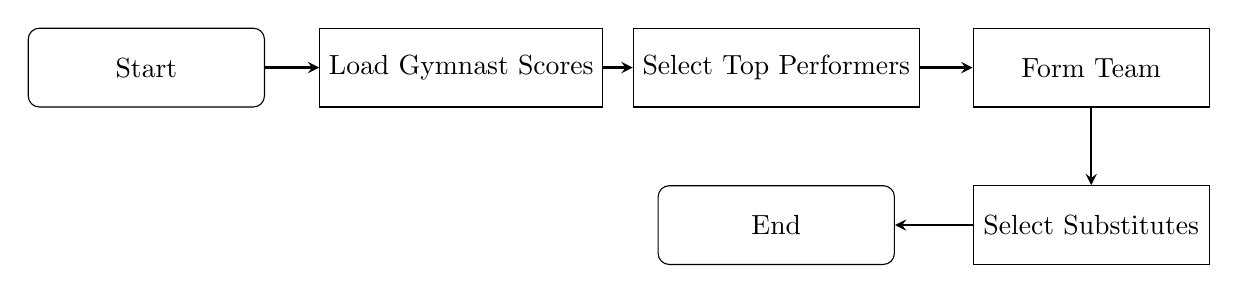
\begin{tikzpicture}[node distance=2cm]
\tikzstyle{startstop} = [rectangle, rounded corners, minimum width=3cm, minimum height=1cm, text centered, draw=black]
\tikzstyle{process} = [rectangle, minimum width=3cm, minimum height=1cm, text centered, draw=black]
\tikzstyle{arrow} = [thick,->,>=stealth]

\node (start) [startstop] {Start};
\node (load) [process, right of=start, xshift=2cm] {Load Gymnast Scores};
\node (select) [process, right of=load, xshift=2cm] {Select Top Performers};
\node (team) [process, right of=select, xshift=2cm] {Form Team};
\node (subs) [process, below of=team] {Select Substitutes};
\node (end) [startstop, left of=subs, xshift=-2cm] {End};

\draw [arrow] (start) -- (load);
\draw [arrow] (load) -- (select);
\draw [arrow] (select) -- (team);
\draw [arrow] (team) -- (subs);
\draw [arrow] (subs) -- (end);

\end{tikzpicture}
\caption{Flowchart for the team selection process}
\end{figure}

\subsubsection{Prediction using Noise}
To simulate the variability and unpredictability in real-world performances, random noise is added to the gymnasts' previous scores. This noise is generated using a Gaussian distribution with a mean of zero and a standard deviation that represents the typical variability in gymnast scores. The exact standard deviation value can be adjusted based on the event and the historical performance data.

\subsubsection{Simulation and Ranking}
Once the noise is added, the gymnasts' scores are used to simulate their performance in the event. Gymnasts are then ranked based on these simulated scores. 

\subsection{Interpreting the Prediction Results}
The results are summarized in a CSV file, which has the following columns:

\begin{table}[H]
    \centering
    \begin{tabular}{|l|l|}
    \hline
    \textbf{Column} & \textbf{Description} \\
    \hline
    Country Names & Names of the participating countries. \\
    \hline
    simulationX & Total number of medals won by the country in the X\textsuperscript{th} simulation. \\
    \hline
    \end{tabular}
    \caption{Description of columns in the result CSV file}
\end{table}

To interpret the results:
\begin{itemize}
    \item Look up the `Country Names` column to identify a specific country.
    \item Check the `simulationX` columns to see the number of medals the country won in each simulation.
    \item The average across all simulation columns provides an estimate of the expected medal count for that country.
\end{itemize}

\subsection{Data Analysis Flowchart}

\begin{figure}[H]
\centering
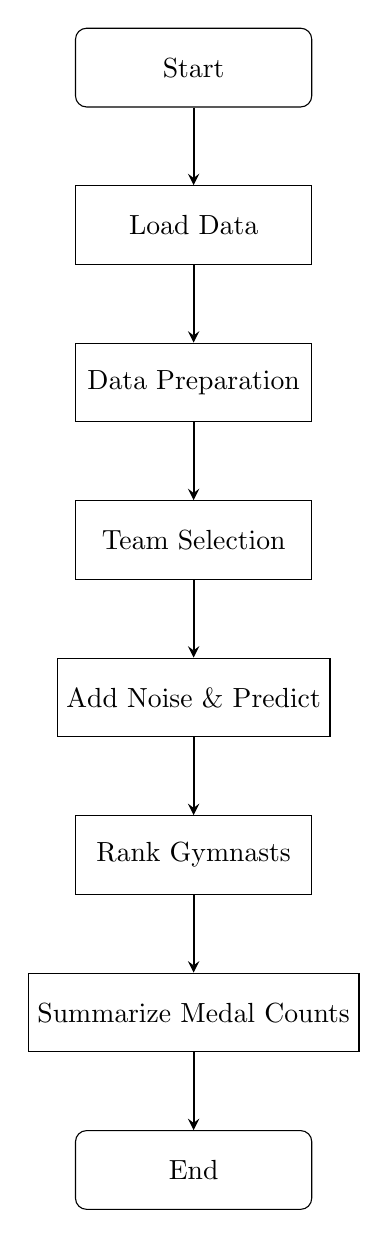
\begin{tikzpicture}[node distance=2cm]
\tikzstyle{startstop} = [rectangle, rounded corners, minimum width=3cm, minimum height=1cm, text centered, draw=black]
\tikzstyle{process} = [rectangle, minimum width=3cm, minimum height=1cm, text centered, draw=black]
\tikzstyle{arrow} = [thick,->,>=stealth]

\node (start) [startstop] {Start};
\node (load) [process, below of=start] {Load Data};
\node (prep) [process, below of=load] {Data Preparation};
\node (teamselect) [process, below of=prep] {Team Selection};
\node (predict) [process, below of=teamselect] {Add Noise \& Predict};
\node (rank) [process, below of=predict] {Rank Gymnasts};
\node (medalcount) [process, below of=rank] {Summarize Medal Counts};
\node (stop) [startstop, below of=medalcount] {End};

\draw [arrow] (start) -- (load);
\draw [arrow] (load) -- (prep);
\draw [arrow] (prep) -- (teamselect);
\draw [arrow] (teamselect) -- (predict);
\draw [arrow] (predict) -- (rank);
\draw [arrow] (rank) -- (medalcount);
\draw [arrow] (medalcount) -- (stop);

\end{tikzpicture}
\caption{Flowchart for the detailed data analysis process}
\end{figure}

\subsection{Conclusion}
The code provides a comprehensive method for analyzing gymnastic data, predicting performance, and summarizing results. It's important to note that the predictions are based on past performance data and include random noise, so they should be interpreted as estimates rather than definitive outcomes.
\end{document}
\bibliographystyle{unsrtnat}
\bibliography{StatisticalCaseStudy.bib}
\end{document}
